\chapter{Preliminaries}

%%%%%%%%%%%%%%%%%%%%%%%%%%%%%%%%
\section{WebGL and its Ancestry}
\summary{Gives an account of WebGL's ancestry (OpenGL, OpenGL ES), motivation, and rapid growth.  Also briefly mentions impediments at the time of writing, such as security concerns and IE support.}

3D graphics in the browser is not new.  One of the first technologies in this area was \index{VRML} VRML, the virtual reality modeling language standardized by the W3C in the mid 90's.  VRML was popular in academia but didn't quite have the same wildfire effect that characterizes the recent explosion of WebGL.

Why has WebGL left other 3D web technologies in the dust?  For one, it came along at just the right time; JavaScript only recently attained status as a serious platform for application development.  Today's world of sophisticated tools like Google's V8 \index{V8} engine  and John Resig's jQuery \index{jQuery} library have legitimized JavaScript in the eyes of developers coming from the world of traditional desktop development.

WebGL has plenty of merits that make it more attractive than other browser-based 3D APIs.  At the time of this writing, almost all popular browsers support it natively, freeing users from the overhead of plug-ins.  WebGL is also ``close to the metal'' -- by providing low-level access to graphics hardware, developers can maximize performance like never before.

WebGL's ancestry actually lies not in VRML (which did give rise to X3D and other XML-based standards) but in a low-level graphics API for C developed by Silicon Graphics in the early 90s.  They initially named their API \emph{IrisGL}, which evolved to \emph{OpenGL} when they released it as an industry standard.   With the rise of mobile platforms, OpenGL spawned \emph{OpenGL ES}, which encompasses almost the same feature set of WebGL.  In a sense, WebGL is simply a JavaScript binding for OpenGL ES 2.0.

WebGL has another ancestor that is arguably just as influential as IrisGL: the \emph{Renderman Shading Language} was developed by Pixar long before the real-time graphics industry could fathom programmable shading.  WebGL gives developers access to an entire programming language known as \index{GLSL} \emph{GLSL}, used to author \index{shaders} \emph{shaders}, relatively small routines executed with massive parallelism.  Shaders have the final say in the 3D position of every vertex, and the RGB color of every rasterized pixel.  We'll learn more about shaders and GLSL in Chapter 2.

%%%%%%%%%%%%%%%%%%%%%%%%%%%%%%%%%%%%%%%%%%%%%
\section{Building Giza}
\summary{Describes our coding conventions and the \code{giza} library that is developed over the course of the book.}

This is not just a book, it's a library.  Much of the sample code on these pages is lifted directly from the \emph{giza} library, named after the city in ancient Egypt.  The skyline of the Giza Necropolis is composed of triangles, the fundamental drawing primitive in computer graphics.  The pyramid shape also describes a \emph{viewing frustum}, a spatial region that encompasses everything within a certain vantage point in a 3D graphics program.

All giza methods belong to a global object called \code{GIZA}; this is a namespacing convention that's very common in JavaScript.  For example, here's how we define a small utility function that merges all attributes from object \code{b} into object \code{a}:

\begin{lstlisting}[language=JavaScript]
var GIZA = GIZA || {};

GIZA.merge = function (a, b) {
  for (var attrname in b) {
    a[attrname] = b[attrname];
  }
};
\end{lstlisting}

The first line allows clients to pick and choose which of Giza's source files to include; it creates a new GIZA object only if it doesn't already exist.  This isn't necessary when using Giza in minified form, since the entire library is included in that case.

The only other global variable is that we ever set is the \code{gl} variable.  This points to a WebGL context, which we'll learn about in Section~\ref{sec:context}.  We chose to make this a global for purposes of terseness, since we make a huge number of calls to the context object.

For access to the full source code to giza, or to download the minified library, refer to our github site:

\notetoself{http://to.be.filled.in.com}

%%%%%%%%%%%%%%%%%%%%%%%%%%%%%%%%%%%%
\section{The Assembly Line Metaphor}
\summary{High-level overview of the WebGL rendering pipeline.}

Hello world how are you.  See Figure~\ref{fig:AssemblyLine}.

\begin{figure}[htb]\centering
  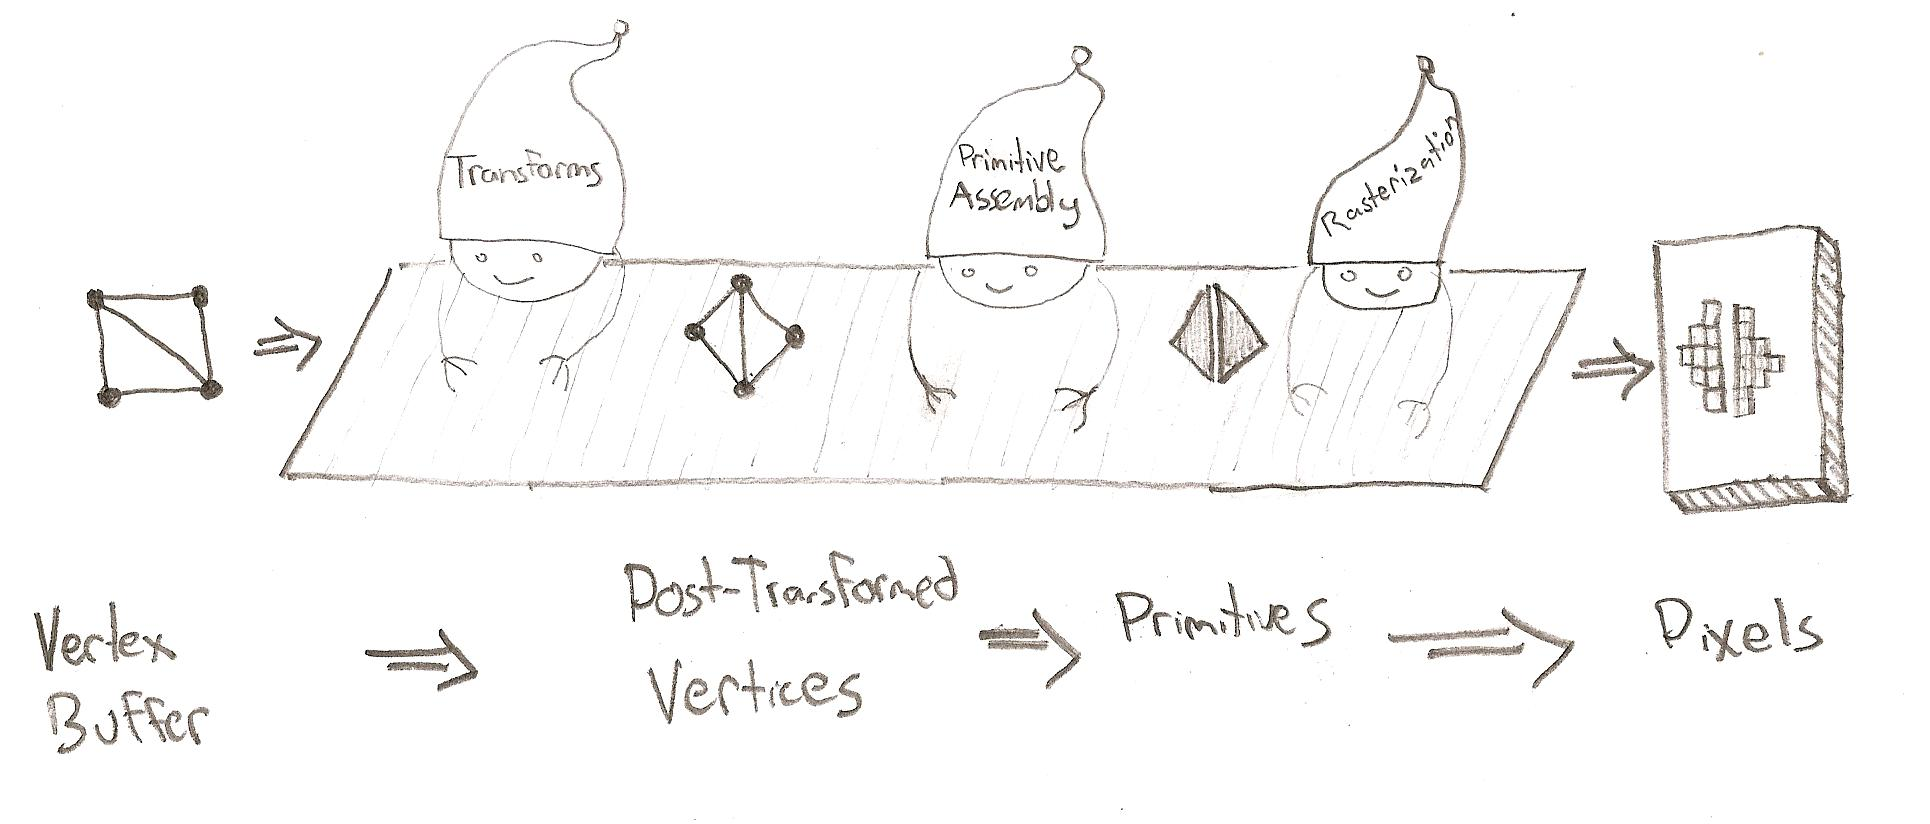
\includegraphics[width=70mm]{AssemblyLine.jpg}
  \caption{In which scenario should you call \code{clear()}?}
  \label{fig:AssemblyLine}
\end{figure}\index{tunnel}

How did you like Figure~\ref{fig:AssemblyLine}?  It was cool no?

%%%%%%%%%%%%%%%%%%%%%%%%%%%%
\section{The Canvas Element}
\summary{Explains the \code{width} and \code{height} attributes and how to handle high-dpi displays (e.g., Apple Retina).}

The canvas element \index{\code{<canvas>} element} is one of the cornerstones of the HTML5 platform.  It provides rich drawing APIs for both 2D and 3D graphics.  The 2D API will not be discussed much in this book (except briefly in Chapter 8), and the 3D API is, of course, WebGL.

\subsection{Dealing with Size}

By default, \code{<canvas>} is a block level element, similar to \code{<div>}.  This means that it can only be a child of \code{<body>}, and that it's typically rendered with surrounding line breaks.

An important distinction between canvas and other elements is that it has two sizes \index{size}.  One size is the \emph{display area}, specified with familiar \index{CSS} CSS mechanisms.  The other size is the \emph{content size}, specified with explicit \code{width} \index{\code{width} attribute} and \code{height} \index{\code{height} attribute} attributes.  The content size specifies an off-screen drawing surface that gets scaled into the display area on the web page.

It's tempting to simply set the content and display sizes to the same dimensions, as in:

\begin{lstlisting}[language=HTML]
<canvas style="width:640px; height:360px"
        width="640" height="360">
</canvas>
\end{lstlisting}

There's nothing wrong with the above approach for simple applications.  It's common, however, to specify a dynamicly-sized display area rather than a fixed one (e.g., \code{width:100\%}).  Moreover CSS pixels don't necessarily correspond to actual device pixels.  This is especially true on displays with a high pixel density, where browsers typically upscale CSS pixels by 2x.

\begin{sidenote}
If you assume that device pixels are 1:1 with CSS pixels, you might see blurriness in your WebGL canvas due to upscaling.
\end{sidenote}

To get around these issues, \code{GIZA.init} \index{\code{GIZA.init}} (Listing~\ref{lst:GIZA:init}) examines the \code{devicePixelRatio} window property to check how much (if any) upscaling the browser is performing.  It also examines the \code{clientWidth} \index{\code{clientWidth}, \code{clientHeight}} and \code{clientHeight} properties of the canvas element to obtain the finalized display area.

\begin{lstlisting}[
    caption={Adjusting the Canvas Size},
    label=lst:GIZA:init,
    language=JavaScript]
GIZA.init = function(canvasElement) {

  // Find a canvas element if one wasn't specified.
  var canvas = canvasElement;
  if (!canvas) {
    canvas = document.getElementsByTagName('canvas')[0];
  }

  // Obtain the browser's upscale amount, assuming 1 if unavailable.
  var pixelScale = window.devicePixelRatio || 1;

  // Define a function that adjusts content size.
  var adjustSize = function() {
    var displayWidth = canvas.clientWidth;
    var displayHeight = canvas.clientHeight;
    canvas.width = displayWidth * pixelScale;
    canvas.height = displayHeight * pixelScale;
  };

  adjustSize();
  window.onresize = adjustSize;
\end{lstlisting}

In Listing~\ref{lst:GIZA:init}, we adjust the canvas width and height not only during initialization, but also during the window's \index{\code{onresize} event} \code{onresize} event.

\begin{sidenote}
It's also common to adjust the WebGL \emph{viewport} and \emph{projection matrix} during a resize event.  More on this in future chapters.
\end{sidenote}

\subsection{Getting a Context}
\label{sec:context}

The entire WebGL API is exposed through a drawing context \index{context} object of type \code{WebGLRenderingContext} \index{\code{WebGLRenderingContext}}.  This object is obtained by calling \code{getContext} \index{\code{getContext} method} on a canvas element, like so:

\begin{lstlisting}[language=JavaScript]
  gl = canvas.getContext('experimental-webgl', {antialias: true});
\end{lstlisting}

At the time of this writing, \code{"experimental-webgl"} \index{\code{experimental-webgl}} is the only string that can be passed to \code{getContext} for WebGL.  (For the 2D canvas API, the string \code{"2d"} is used.)

The second argument is a set of optional attributes, as specified in Table~\ref{tab:ContextAttributes}.

\begin{table}[htb]\centering
  \begin{tabular}{lll}
    \hline
    Key & Default Value & Description \\
    \hline
    alpha & true & Alpha channel \\
    depth & true & Depth buffer \\
    stencil & false & Stencil buffer \\
    antialias & true & Enables multisampling (or supersampling) \\
    premultipliedAlpha & true & Specifies compositing behavior with the web page; ignored if alpha is false \\
    preserveDrawingBuffer & false & Retains the canvas image from the previous draw cycle \\
    \hline
  \end{tabular}
  \caption{WebGL Context Options.}
  \label{tab:ContextAttributes}
\end{table}

We'll examine these attributes in Table~\ref{tab:ContextAttributes} in greater detail in the next section.

\notetoself{Add references to future sections in the book that deal with context loss and image capture.}

\subsection{Clearing the Canvas}

The only WebGL functions we're discussing in this chapter are the first two methods listed in Table~\ref{tab:Clearing}.

\begin{table}[htb]\centering
  \begin{tabular}{ll}
    \hline
    Method & Argument Types \\
    \hline
    clear(mask) & logical or of values in Table~\ref{tab:ClearBits} \\
    clearColor(red, green, blue, alpha)  & floating point numbers in [0,1] \\
    clearDepth(value) & floating point number in [0,1] \\
    clearStencil(mask) & integer \\
    \hline
  \end{tabular}
  \caption{WebGL Clear Methods.}
  \label{tab:Clearing}
\end{table}

The \code{clear} command has an immediate\footnote{It's actually not quite immediate -- see \label{sec:doublebuffer}.} effect on the canvas, while \code{clearColor}, \code{clearDepth}, and \code{clearStencil} are simply configuring the WebGL state machine.  Most of the WebGL API consists of state-setting commands; there are only three methods in the entire API that can draw pixels into your canvas:

\begin{itemize}
\item clear
\item drawArrays
\item drawElements
\end{itemize}

We'll learn more about \code{drawArrays} and \code{drawElements} in the next chapter.  Listing~\ref{lst:ClearCanvas} shows a typical usage pattern for the \code{clear} method.

\begin{lstlisting}[
    caption={Clearing the canvas},
    label=lst:ClearCanvas,
    language=JavaScript]
gl = canvas.getContext('experimental-webgl', {antialias: true});
gl.clearColor(1, 1, 0, 1);
gl.clear(gl.COLOR_BUFFER_BIT);
\end{lstlisting}

The \code{COLOR\_BUFFER\_BIT} flag is one of the constants that can be combined with a logical ``or'' to specify which drawing layers to include in the canvas.  To reduce the memory footprint, choose the fewest number of required flags.  See tab:ClearBit.  Don't worry about the depth and stencil layers; we'll learn more about them in future chapters.

\begin{table}[htb]\centering
  \begin{tabular}{lll}
    \hline
    Property & Value & Default Value \\
    \hline
    \code{DEPTH\_BUFFER\_BIT}   & 0x0100 & 0.0 \\
    \code{STENCIL\_BUFFER\_BIT} & 0x0400 & 0x00000000\\
    \code{COLOR\_BUFFER\_BIT}   & 0x4000 & (0, 0, 0, 0) \\
    \hline
  \end{tabular}
  \caption{WebGL Clear Bits.}
  \label{tab:ClearBit}
\end{table}

You can find a \code{clear} call in many WebGL code samples on the web, but keep in mind that it's not always required.  Some applications never bother filling the background with a solid color; for example, consider an ``infinite tunnel'' game, as depicted on the far left in Figure~\ref{fig:Tunnel}.  Since every pixel in the canvas is affected by 3D drawing commands, there's no need to clear the color buffer.  If, however, the tunnel were finite (middle panel, Figure~\ref{fig:Tunnel}), there would be an area of the screen that never gets drawn to.  If you don't explicitly perform a clear before doing any drawing, the unpainted region might contain a ``dirty'' image (right panel, Figure~\ref{fig:Tunnel}), depending on the \code{preserveDrawingBuffer} option you chose when creating the context.

\begin{figure}[htb]\centering
  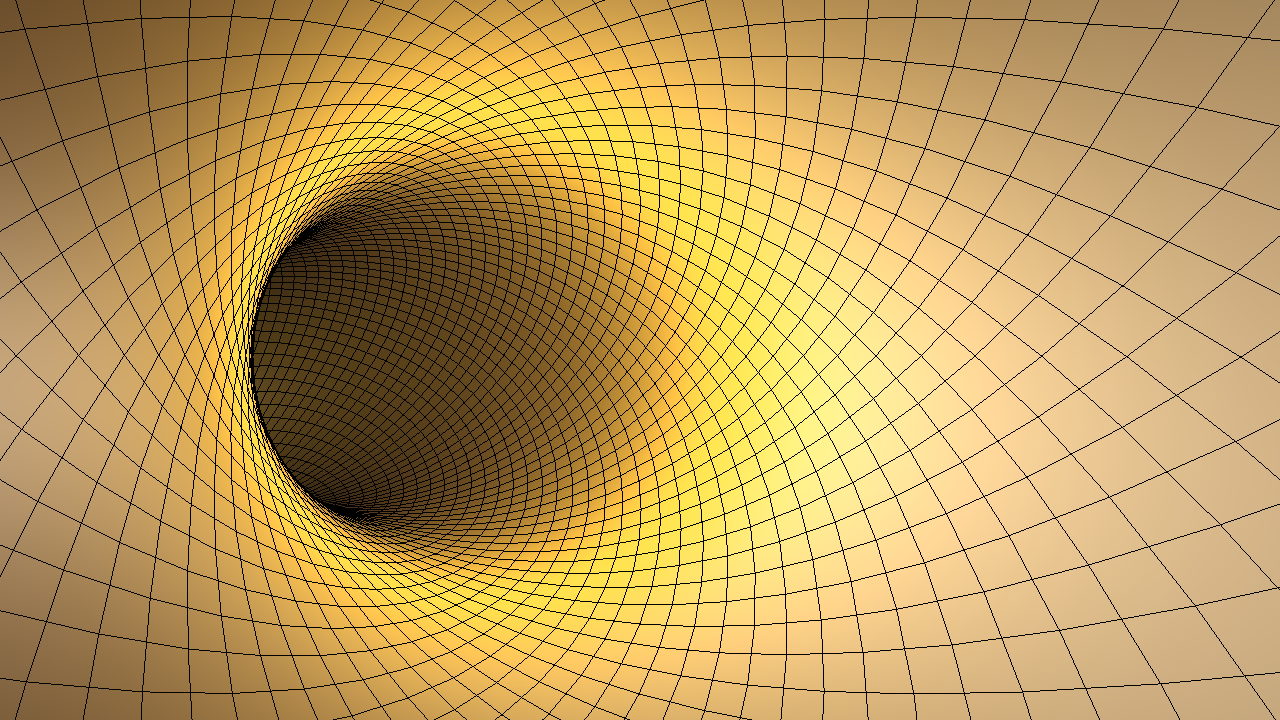
\includegraphics[width=70mm]{ClosedTunnel.png}
  \caption{In which scenario should you call \code{clear()}?}
  \label{fig:Tunnel}
\end{figure}\index{tunnel}

\subsection{When is the canvas \emph{truly} updated?}
\label{sec:doublebuffer}

You might be familiar with \index{double-buffering} \emph{double-buffering} if you've used other graphics APIs.  WebGL is always double-buffered.  This means that your drawing commands are actually affecting pixels in a \index{backbuffer} \emph{backbuffer}, which is an offscreen drawing surface.  The browser's render loop presents the finalized backbuffer to the screen in one fell swoop.  This creates the illusion of seamless animation; users never see a partially complete scene.

Double-buffering implies that the existing pixels you're drawing on top of do not correspond to what was drawn in the previous frame.  Normally this doesn't matter; most applications either clear the existing buffer, or fill it entirely with 3D drawing primitives.

In some situations you want the existing pixels to exactly correspond to the previously-drawn frame.  For example, you might need to read color values from the canvas (the \index{\code{readPixels}} \code{readPixels} method will be discussed in \notetoself{CHAPTER}), or your application might intentionally update only certain regions of the canvas, perhaps for performance reasons.  This is why \code{preserveDrawingBuffer} exists; it allows you to mimic \index{single-buffering} single-buffering.

You might be thinking: \emph{okay -- the backbuffer is what's immediately updated when I call \code{clear} or \code{drawPixels}}.  Wrong!  The web browser and the graphics driver are actually buffering up WebGL commands and executing them later.  If you'd like, you can tell WebGL to wait till the buffer is done executing by calling the \index{finish} \code{finish} method.  You'll rarely need to use this however, so don't do it unless you really need to.

\subsection{Alpha Compositing}

If you're reading this book, you're probably already familiar with the concept of an alpha channel, invented in the late 70's by Alvy Ray Smith, one of the co-founders of the animation studio where I work.

Briefly, alpha is a floating-point value in the [0,1] interval, treated much like the red, green, and blue components of pixel color.  Alpha can be thought of as the inverse of opacity, although WebGL can interpret it in many ways, as we'll learn in Chapter \notetoself{CHAPTER}.  For now we'll focus on the existence of the alpha channel in the canvas and how it interacts with the HTML page compositor in your browser.

PAGECOMPOSITOR

\begin{comment}
images of a web page that has a background image (Egypt!)
each canvas should have an opaque perspective cube

0,0.25,.5,.5 -- no alpha, css-opacity=1
0,0.25,.5,.5 -- alpha without premultiplied, css-opacity=1
0,0.25,.5,.5 -- alpha with premultiplied, css-opacity=1

0,0.25,.5,.5 -- no alpha, css-opacity=.5
0,0.25,.5,.5 -- alpha without premultiplied, css-opacity=.5
0,0.25,.5,.5 -- alpha with premultiplied, css-opacity=.5
\end{comment}

\begin{sidenote}
In this book, we never add children elements to \code{<canvas>}, but there's nothing wrong with doing so.  On some platforms, this can degrade performance, although this is improving as WebGL implementations are maturing.
\end{sidenote}

...

%%%%%%%%%%%%%%%%%%%%%%%%%%
\section{Animation Timing}
\summary{How to periodically trigger draw events.}

\begin{lstlisting}[language=JavaScript]
  window.requestAnimationFrame = window.requestAnimationFrame ||
    window.mozRequestAnimationFrame ||
    window.webkitRequestAnimationFrame ||
    window.msRequestAnimationFrame;
\end{lstlisting}

%%%%%%%%%%%%%%%%%%%%%%%%%%%%%%%%
\rrecipe{Recipe 1: Strobe Light}
\summary{The simplest possible WebGL application; animates a solid color with \code{clear}.}

